\question \textbf{Matching n-grams}
  
Calculate the scores of the segment pairs between q: CG and all 2-gram permutations of \{A, C, G, T\}.

\medskip 

Score matrix:
\begin{figure}[H]
      \centering
      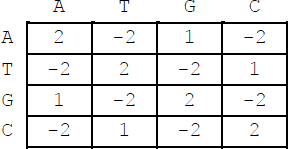
\includegraphics[width=0.25 \textwidth]{fig05/score_scheme_1.png}
\end{figure}

\vspace{0.1 in}

\begin{parts}

%% (a)
  \part Fill the scores between CG and all its matching n-grams.

\begin{figure}[H]
      \centering
      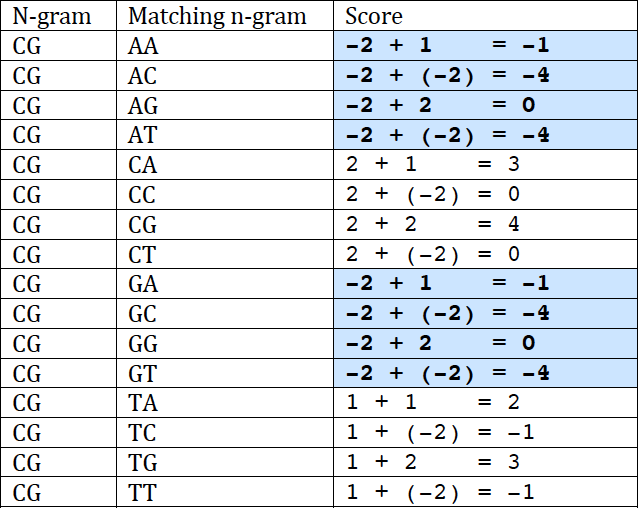
\includegraphics[width=0.6 \textwidth]{fig05/matching_n-gram_solution.png}
\end{figure}

%% (b)
\part Identify all matching n-grams when the threshold value T is 3.

\begin{solution}[0.5 in]
\begin{verbatim}
  CA, CG, TG
\end{verbatim}
\end{solution}

\end{parts}

